\documentclass[ngerman,]{article}
\usepackage[sfdefault]{roboto}
\usepackage{amssymb,amsmath}
\usepackage{ifxetex,ifluatex}
\usepackage{fixltx2e} % provides \textsubscript
\ifnum 0\ifxetex 1\fi\ifluatex 1\fi=0 % if pdftex
  \usepackage[T1]{fontenc}
  \usepackage[utf8]{inputenc}
\else % if luatex or xelatex
  \ifxetex
    \usepackage{mathspec}
  \else
    \usepackage{fontspec}
  \fi
  \defaultfontfeatures{Ligatures=TeX,Scale=MatchLowercase}
\fi
% use upquote if available, for straight quotes in verbatim environments
\IfFileExists{upquote.sty}{\usepackage{upquote}}{}
% use microtype if available
\IfFileExists{microtype.sty}{%
\usepackage[]{microtype}
\UseMicrotypeSet[protrusion]{basicmath} % disable protrusion for tt fonts
}{}
\PassOptionsToPackage{hyphens}{url} % url is loaded by hyperref
\usepackage[unicode=true]{hyperref}
\PassOptionsToPackage{usenames,dvipsnames}{color} % color is loaded by hyperref
\hypersetup{
            pdftitle={Anforderungsanalyse},
            pdfauthor={Andreas Saurer; Benjamin Schneidinger; Josef Erben; Raffaele Bof; Nicolas Loth},
            colorlinks=true,
            linkcolor=[RGB]{74,144,226},
            citecolor=[RGB]{74,144,226},
            urlcolor=[RGB]{74,144,226},
            breaklinks=true}
\urlstyle{same}  % don't use monospace font for urls
% \usepackage[1]{geometry}
\usepackage[a4paper,top=45mm,right=20mm,bottom=30mm,left=25mm,head=35mm,foot=20mm]{geometry}
\ifnum 0\ifxetex 1\fi\ifluatex 1\fi=0 % if pdftex
  \usepackage[shorthands=off,main=ngerman]{babel}
\else
  \usepackage{polyglossia}
  \setmainlanguage[]{german}
\fi
\usepackage{longtable,tabu,booktabs}
% Fix footnotes in tables (requires footnote package)
\IfFileExists{footnote.sty}{\usepackage{footnote}\makesavenoteenv{long table}}{}
\usepackage{graphicx,grffile}
\graphicspath{ {docs/images/} }
\makeatletter
\def\maxwidth{\ifdim\Gin@nat@width>\linewidth\linewidth\else\Gin@nat@width\fi}
\def\maxheight{\ifdim\Gin@nat@height>\textheight\textheight\else\Gin@nat@height\fi}
\makeatother
% Scale images if necessary, so that they will not overflow the page
% margins by default, and it is still possible to overwrite the defaults
% using explicit options in \includegraphics[width, height, ...]{}
\setkeys{Gin}{width=\maxwidth,height=\maxheight,keepaspectratio}
\IfFileExists{parskip.sty}{%
\usepackage{parskip}
}{% else
\setlength{\parindent}{0pt}
\setlength{\parskip}{6pt plus 2pt minus 1pt}
}
\setlength{\emergencystretch}{3em}  % prevent overfull lines
\providecommand{\tightlist}{%
  \setlength{\itemsep}{0pt}\setlength{\parskip}{0pt}}
\setcounter{secnumdepth}{5}
% % % Redefines (sub)paragraphs to behave more like sections
% \ifx\paragraph\undefined\else
% \let\oldparagraph\paragraph
% \renewcommand{\paragraph}[1]{\oldparagraph{#1}\mbox{}}
% \fi
% \ifx\subparagraph\undefined\else
% \let\oldsubparagraph\subparagraph
% \renewcommand{\subparagraph}[1]{\oldsubparagraph{#1}\mbox{}}
% \fi
% 
% header and footer
\usepackage{lastpage}
\usepackage{fancyhdr}
\pagestyle{fancy}
\fancyhf{}
\fancyhead[L]{
\includegraphics[height=2cm]{travel-buddy_white.png}}
\fancyfoot[L]{\fontsize{8}{10}\selectfont\ Anforderungsanalyse}
\fancyfoot[R]{\fontsize{8}{10}\selectfont\ Seite\ \thepage\ von\ \pageref*{LastPage}}

\renewcommand{\headrulewidth}{0pt}
\renewcommand{\footrulewidth}{0pt}

% style titles
\usepackage{titlesec}
\titlespacing*{\section}{0pt}{1em}{0pt}
\titlespacing*{\subsection}{0pt}{1em}{0pt}
\titlespacing*{\subsubsection}{0pt}{1em}{0pt}

% set default figure placement to htbp
\makeatletter
\def\fps@figure{htbp}
\makeatother


\title{
\includegraphics[width=7cm]{travel-buddy_white.png}\\Anforderungsanalyse}
\author{Andreas Saurer \\ Benjamin Schneidinger \\ Josef Erben \\ Raffaele Bof \\ Nicolas Loth}
      \date{\parbox{\linewidth}{\centering%
      IT15TA ZH \hspace*{3cm} Gruppe 3\endgraf\bigskip
      28.03.2017\endgraf
    }}
  
\begin{document}
\maketitle
\newpage

{
\hypersetup{linkcolor=black}
\setcounter{tocdepth}{3}
\tableofcontents
}
\newpage
\section{Versionenlog}\label{versionenlog}

\tabulinesep=1.2mm

\begin{longtabu} to \textwidth { | l | l | l | X[l] | }
  \hline
  \textbf{Datum} & \textbf{Version} & \textbf{Änderung} & \textbf{Author} \\
  \hline
  \endhead

  0.0.3 & 21.03.2017 & Anwendungsfalldiagramm hinzugefügt & Benjamin Schneidinger\\
  \hline

  0.0.2 & 21.03.2017 & Zusätzliche Spezifikationen definiert & Benjamin Schneidinger\\
  \hline

  0.0.1 & 21.03.2017 & Anwendungsfälle beschrieben und Systemsequenzdiagramm eingebunden & Andreas Saurer\\
  \hline

  0.0.0 & 21.03.2017 & Dokument erstellt & Andreas Saurer\\
  \hline
\end{longtabu}\newpage

\section{Projektmanagement}\label{projektmanagement}

\subsection{Projektstatus}\label{projektstatus}

Das Projekt befindet sich auf Kurs, der erste Meilenstein wurde erreicht
und der zweite bevorstehende Meilenstein ist fast fertig gestellt. Die
unten gezeigte Grafik zeigt eine grobe Übersicht des Projektes, eine
detaillierte befindet sich im darauf folgenden Abschnitt.

\begin{figure}
\centering
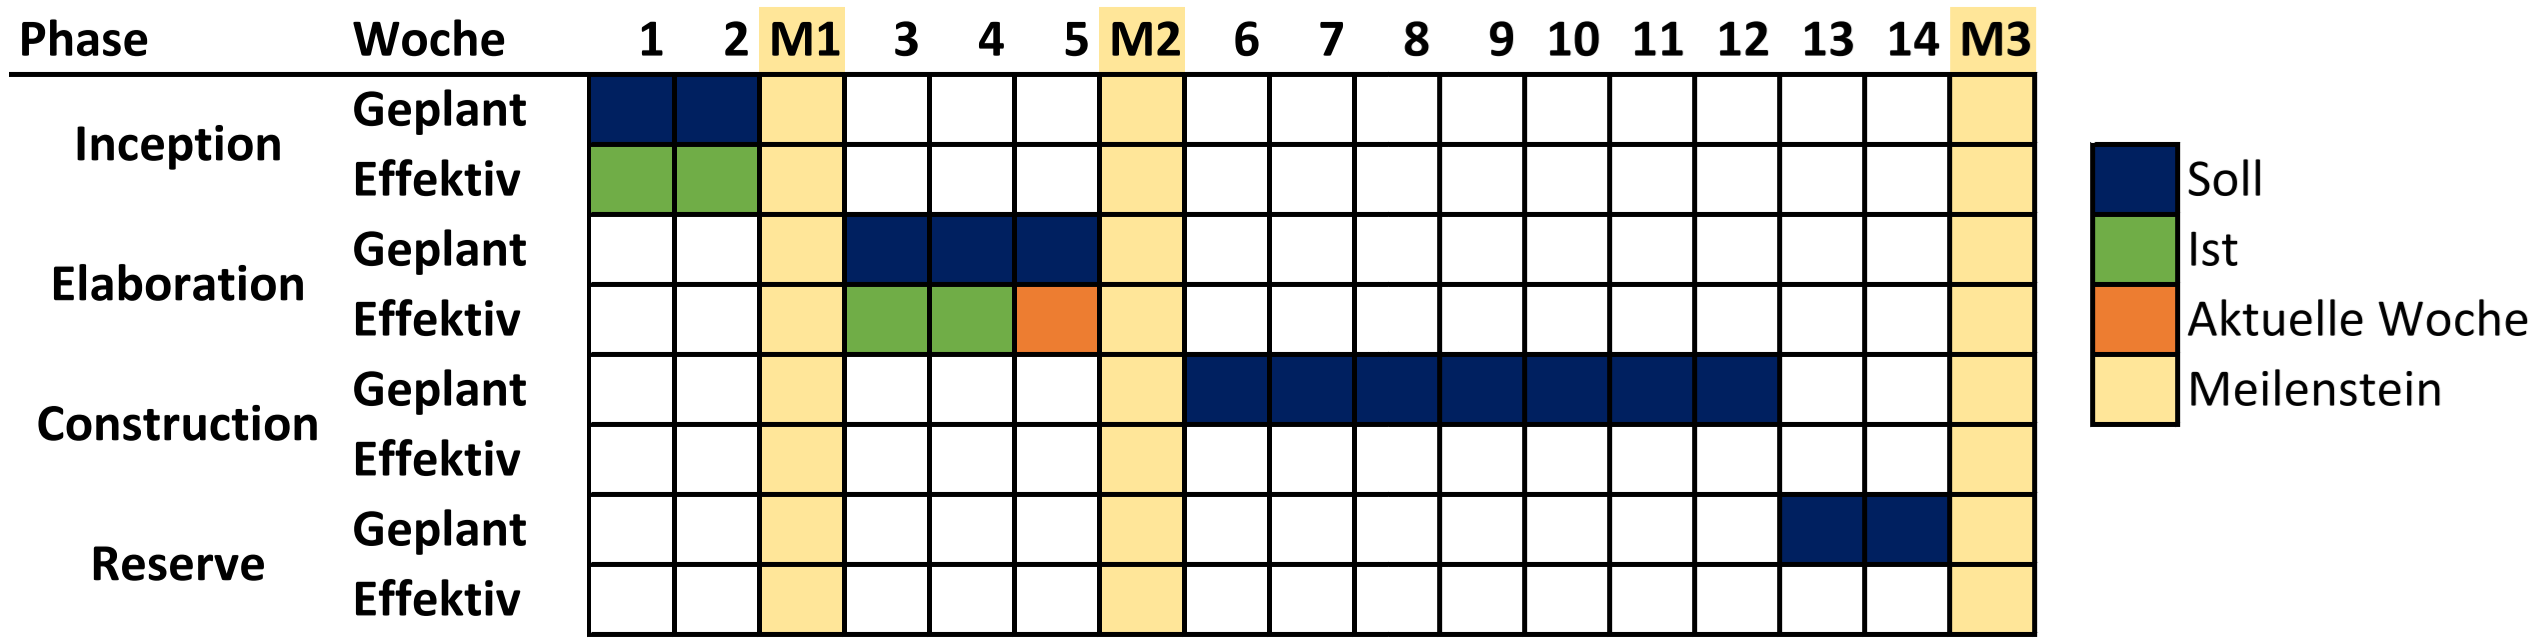
\includegraphics{https://raw.githubusercontent.com/PsitTeam3/Documentation/master/docs/diagrams/Grobzeitplan_26.03.2017.png}
\caption{Grobzeitplan Stand:26.03.2017}
\end{figure}

\subsection{Detaillierter Projektplan}\label{detaillierter-projektplan}

\begin{longtable}[]{@{}lccrr@{}}
\toprule
\textbf{Phase} & \textbf{NR} & \textbf{Arbeitspaket} & \textbf{Soll} &
\textbf{Ist}\tabularnewline
\midrule
\endhead
Inception & & & &\tabularnewline
& A-01 & Ausgangslage schildern & 5,0 h &\tabularnewline
& A-02 & Projektidee beschreiben & 5,0 h &\tabularnewline
& A-03 & Kundennutzen analysieren & 5,0 h &\tabularnewline
& A-04 & Projektidee beschreiben & 5,0 h &\tabularnewline
& A-05 & Konkurenzanalyse & 5,0 h &\tabularnewline
& A-06 & Haupablauf aufzeigen & 5,0 h &\tabularnewline
& A-07 & Weitere Anforderungen definieren & 5,0 h &\tabularnewline
& A-08 & Ressource beschreiben & 5,0 h &\tabularnewline
& A-09 & Projektidee beschreiben & 5,0 h &\tabularnewline
& A-10 & Risiken beschreiben & 5,0 h &\tabularnewline
& A-11 & Grobplanung erstellen & 5,0 h & 3,5 h\tabularnewline
& A-12 & Wirtschaftlichkeitsanalyse & 5,0 h & 6,0 h\tabularnewline
& A-13 & Projektskizze erstellen (inkl. Präsi) & 5,0 h &\tabularnewline
Total Phase: & 13 & & 65,0 h &\tabularnewline
Inception & & & &\tabularnewline
& B-01 & Projekmanagement organisieren & 5,0 h & 6,0 h\tabularnewline
& B-02 & Anwendungsfall Diagramm zeichnen & 5,0 h &\tabularnewline
& B-03 & Domänenmodell erstellen & 5,0 h &\tabularnewline
& B-04 & Architektur beschreiben & 5,0 h &\tabularnewline
& B-05 & Zusätzliche Spezifikationen beschreiben & 5,0 h
&\tabularnewline
& B-06 & Syste-Sequenzdiagramm zeichnen & 5,0 h &\tabularnewline
& B-07 & Glossar erstellen & 5,0 h &\tabularnewline
& B-08 & Use-Case 1 beschreiben & 1,0 h &\tabularnewline
& B-09 & Use-Case 2 beschreiben & 0,5 h &\tabularnewline
& B-10 & Use-Case 3 beschreiben & 0,5 h &\tabularnewline
& B-11 & Use-Case 4 beschreiben & 0,5 h &\tabularnewline
& B-12 & Use-Case 5 beschreiben & 0,5 h &\tabularnewline
& B-13 & Use-Case 6 beschreiben & 0,5 h & 0,5 h\tabularnewline
& B-14 & Analysedokument erstellen (inkl. Präsi) & 6,5 h
&\tabularnewline
Total Phase: & 14 & & 45,0 h &\tabularnewline
Construction & & & &\tabularnewline
& C-01 & Projekmanagement nachtragen & 1,0 h &\tabularnewline
& C-02 & UC-1 Liste der verfügbaren Touren & ? h &\tabularnewline
& C-03 & UC-1 Starten einer Tour & ? h &\tabularnewline
& C-04 & UC-2 Lokalisieren des Benutzers & ? h &\tabularnewline
& C-05 & UC-2 Anzeigen des Benutzers auf der Karte & ? h
&\tabularnewline
& C-06 & UC-3 Foto machen & ? h &\tabularnewline
& C-07 & UC-4 Prüfen der Geo koordinaten des Fotos & ? h
&\tabularnewline
& C-08 & UC-5 Besuchen des nächsten Punktes & ? h &\tabularnewline
& C-09 & UC-6 Auslesen der Tourdaten & ? h &\tabularnewline
& C-10 & UC-6 Anzeigen der Tourdaten & ? h &\tabularnewline
& C-11 & UI gestalten & ? h &\tabularnewline
& C-12 & Systemtests durchführen & ? h &\tabularnewline
& C-13 & Dokumentation erstellen & ? h &\tabularnewline
& C-14 & Benutzeranleitung schreiben & ? h &\tabularnewline
Total Phase: & 14 & & ? h &\tabularnewline
\bottomrule
\end{longtable}

\subsection{Risiken}\label{risiken}

\begin{longtable}[]{@{}rcrr@{}}
\toprule
\begin{minipage}[b]{0.06\columnwidth}\raggedleft\strut
\textbf{NR}\strut
\end{minipage} & \begin{minipage}[b]{0.50\columnwidth}\centering\strut
\textbf{Risiko}\strut
\end{minipage} & \begin{minipage}[b]{0.14\columnwidth}\raggedleft\strut
\textbf{Auswirkung}\strut
\end{minipage} & \begin{minipage}[b]{0.19\columnwidth}\raggedleft\strut
\textbf{Wahrscheinlichkeit}\strut
\end{minipage}\tabularnewline
\midrule
\endhead
\begin{minipage}[t]{0.06\columnwidth}\raggedleft\strut
1\strut
\end{minipage} & \begin{minipage}[t]{0.50\columnwidth}\centering\strut
Schutz der gespeicherten Daten durch unauthorisierte Zugriffe\strut
\end{minipage} & \begin{minipage}[t]{0.14\columnwidth}\raggedleft\strut
Schwerwiegend\strut
\end{minipage} & \begin{minipage}[t]{0.19\columnwidth}\raggedleft\strut
Hoch\strut
\end{minipage}\tabularnewline
\begin{minipage}[t]{0.06\columnwidth}\raggedleft\strut
2\strut
\end{minipage} & \begin{minipage}[t]{0.50\columnwidth}\centering\strut
Hohe kosten für Anwender Aufgrund der verwendung durch
Kartenmaterial\strut
\end{minipage} & \begin{minipage}[t]{0.14\columnwidth}\raggedleft\strut
Mittel\strut
\end{minipage} & \begin{minipage}[t]{0.19\columnwidth}\raggedleft\strut
Hoch\strut
\end{minipage}\tabularnewline
\begin{minipage}[t]{0.06\columnwidth}\raggedleft\strut
3\strut
\end{minipage} & \begin{minipage}[t]{0.50\columnwidth}\centering\strut
Fehlendes Wissen in der Entwicklung von Mobile Apps\strut
\end{minipage} & \begin{minipage}[t]{0.14\columnwidth}\raggedleft\strut
Mittel\strut
\end{minipage} & \begin{minipage}[t]{0.19\columnwidth}\raggedleft\strut
Mittel\strut
\end{minipage}\tabularnewline
\begin{minipage}[t]{0.06\columnwidth}\raggedleft\strut
4\strut
\end{minipage} & \begin{minipage}[t]{0.50\columnwidth}\centering\strut
Höhere komplexität durch einbinden von 3 Anbieter Software\strut
\end{minipage} & \begin{minipage}[t]{0.14\columnwidth}\raggedleft\strut
Gering\strut
\end{minipage} & \begin{minipage}[t]{0.19\columnwidth}\raggedleft\strut
Mittel\strut
\end{minipage}\tabularnewline
\begin{minipage}[t]{0.06\columnwidth}\raggedleft\strut
5\strut
\end{minipage} & \begin{minipage}[t]{0.50\columnwidth}\centering\strut
Keine öffentlichen Karten-API verfügbar\strut
\end{minipage} & \begin{minipage}[t]{0.14\columnwidth}\raggedleft\strut
Schwerwiegend\strut
\end{minipage} & \begin{minipage}[t]{0.19\columnwidth}\raggedleft\strut
Sehr gering\strut
\end{minipage}\tabularnewline
\begin{minipage}[t]{0.06\columnwidth}\raggedleft\strut
6\strut
\end{minipage} & \begin{minipage}[t]{0.50\columnwidth}\centering\strut
Smartphone GPS koordination ungenau\strut
\end{minipage} & \begin{minipage}[t]{0.14\columnwidth}\raggedleft\strut
Gering\strut
\end{minipage} & \begin{minipage}[t]{0.19\columnwidth}\raggedleft\strut
Mittel\strut
\end{minipage}\tabularnewline
\bottomrule
\end{longtable}

\section{Anwendungsfälle}\label{anwendungsfuxe4lle}

\subsection{UC 1: User wählt Tour aus und startet die Tour (Priorität
1)}\label{uc-1-user-wuxe4hlt-tour-aus-und-startet-die-tour-priorituxe4t-1}

\subsubsection{Primärer Akteur}\label{primuxe4rer-akteur}

Benutzer

\subsubsection{Stakeholders und
Interessen}\label{stakeholders-und-interessen}

\begin{itemize}
\tightlist
\item
  Benutzer: Will mit einfachen Schritten eine passende Tour finden und
  starten
\item
  Premium Tour Anbieter: Will seine Tour prominent plaziert haben um
  öfters ausgewählt zu werden
\end{itemize}

\subsubsection{Vorbedingungen}\label{vorbedingungen}

\begin{itemize}
\tightlist
\item
  Benutzer ist angemeldet
\item
  Touren sind auf Server erfasst
\end{itemize}

\subsubsection{Erfolgsgarantie}\label{erfolgsgarantie}

Benutzer findete eine ansprechende Tour und kann diese starten

\subsubsection{Standardablauf}\label{standardablauf}

\begin{enumerate}
\def\labelenumi{\arabic{enumi}.}
\tightlist
\item
  Benutzer öffnet app
\item
  Benutzer klickt auf neue Tour starten
\item
  App zeigt Auswahl von Touren
\item
  Benutzer öffnet Filter
\item
  Benutzer setzt Filter um gewünschte Tour zu finden
\item
  Benutzer klickt auf Tour
\item
  Tour wird gestartet
\item
  Der Benutzer begibt sich zum Startpunkt der Tour
\end{enumerate}

\subsubsection{Erweiterungen}\label{erweiterungen}

3a. Auswahl ist abhängig von gerade populären oder von Premium Anbietern
beworbenen Touren\newline
6a. App zeigt Detailvorschau an\newline
6b. Benutzer klickt auf Tour starten oder schliessen\newline
8a. Die App zeigt dem Benutzer verschiedene Möglichkeiten an, wie er zum
Startpunkt kommt.

\subsubsection{Spezielle Anforderungen}\label{spezielle-anforderungen}

\begin{itemize}
\tightlist
\item
  Filtern der Touren muss flüssig reagieren, Resultate werden sofort
  angezeigt
\end{itemize}

\subsubsection{Auftrittshäufigkeit}\label{auftrittshuxe4ufigkeit}

Einmal pro Tour

\subsection{UC 2: User läuft Route ab und sieht seine aktuellen Standort
auf einer Karte (Priorität
2)}\label{uc-2-user-luxe4uft-route-ab-und-sieht-seine-aktuellen-standort-auf-einer-karte-priorituxe4t-2}

\subsubsection{Erfolgszenario}\label{erfolgszenario}

Der Tourist befindet sich im Freien zwischen zwei Punkten auf einer
Route, also einer Teilstrecke der Tour. Die App zeigt dem Benutzer seine
aktuelle Position mit einem Marker (z.B. Punkt) an. Der User verlässt
die Route, der Marker zeigt in Echtzeit die Position an, an der er sich
befindet. Die App berechnet die neue Route mit der aktuellen Postion als
Ausgangslage. Der User kann also zu jederzeit die optimale Route
zwischen seiner aktuellen Position und dem Ziel nachschauen.

\subsubsection{Erfolgszenario mit
Fallback}\label{erfolgszenario-mit-fallback}

Der Tourist befindet sich auf einer Tour durch eine Altstadt. Die App
zeigt dem Benutzer seine aktuelle Position mit einem Marker (z.B. Punkt)
an, der Marker bewegt sich mit dem User mit. Die aktuelle Route zum
nächsten Zwischenziel führt durch ein dicht überdachtes Gebiet. Die App
kann die Position des Users nicht per GPS abfragen, in der Nähe stehen
einige Läden und Restaurants mit WLAN. Die App kann durch eine
Kombination von Standorten von Mobilfunkmasten und WLAN Sendern die
aktuelle Position berechnen. Der Benutzer hat kein GPS Signal, aber
sieht sich trotzdem als Punkt auf der Karte in Echtzeit.

\subsection{UC 3: User macht Foto am Besichtigungspunkt (Priorität
2)}\label{uc-3-user-macht-foto-am-besichtigungspunkt-priorituxe4t-2}

\subsubsection{Erfolgszenario}\label{erfolgszenario-1}

An einem Zielpunkt / Besichtigungspunkt angelangt, wird der Benutzer
aufgefordert, ein Foto von einem vorgegebenen Objekt zu erstellen. Die
App entscheidet danach ob die Informationen des Fotos mit denjenigen im
System gespeicherten übereinstimmen. Stimmt das Resultat, wird der
nächste Besichtigungspunkt angezeigt.

\subsubsection{Alternativszenario}\label{alternativszenario}

Befindet sich der Benutzer nicht am korrekten Ort, wird er erneut
aufgefordert das vorgegebene Objekt zu fotografieren.

\subsection{UC 4: User bekommt Bestätigung für das Abarbeiten des
Punktes, die Route zum nächsten Punkt wird angezeigt. (Priorität
2)}\label{uc-4-user-bekommt-bestuxe4tigung-fuxfcr-das-abarbeiten-des-punktes-die-route-zum-nuxe4chsten-punkt-wird-angezeigt.-priorituxe4t-2}

\subsubsection{Erfolgszenario}\label{erfolgszenario-2}

Nach dem korrekten validieren der Position des Touristen, zeigt die App
dem Benutzer den nächsten Besichtigungspunkt mit einem Marker auf einer
Karte an. Von seinem aktuellen Standort wird eine vordefinierte Route
zum nächsten Besichtigungspunkt abgebildet. Der Tourist begiebt sich zum
abgebildeten Punkt.

\subsubsection{Alternativszenario}\label{alternativszenario-1}

Der Benutzer möchte die Tour unterbrechen und zu einem späteren
Zeitpunkt fortsetzen. Er schliesst die App und kehrt nach unbestimmter
Zeit zurück. Die App zeigt dann den letzten Stand und fragt nach der
Weiterführung oder Abbruch der Tour.

\subsection{UC 5: User besucht nächste Punkte bis Tour zu Ende.
(Priorität
2)}\label{uc-5-user-besucht-nuxe4chste-punkte-bis-tour-zu-ende.-priorituxe4t-2}

UC1 und UC2 werden solange wiederholt, bis der Tourist am Ende der Tour
ist. Hat er den letzten Punkt erreicht, wird dem Benutzer der Abschluss
mit einer Nachricht bestätigt und mit UC 6 fortgefahren.

\subsection{UC 6: User sieht Statistik der Tour. (Priorität
3)}\label{uc-6-user-sieht-statistik-der-tour.-priorituxe4t-3}

Nach erfolgreichem erreichen des Zielpunktes und dem Abschluss der Tour,
wird dem Benutzer eine übersicht mit Statistiken wie z.B. der total
zurück gelegten Distanz und totale Schritte angezeigt. Durch einen klick
kann der Benutzer Fotos, die Statistik und eine Mitteilung auf den
sozialen Medien teilen.

\section{Anwendungsfalldiagramm}\label{anwendungsfalldiagramm}

\begin{figure}
\centering
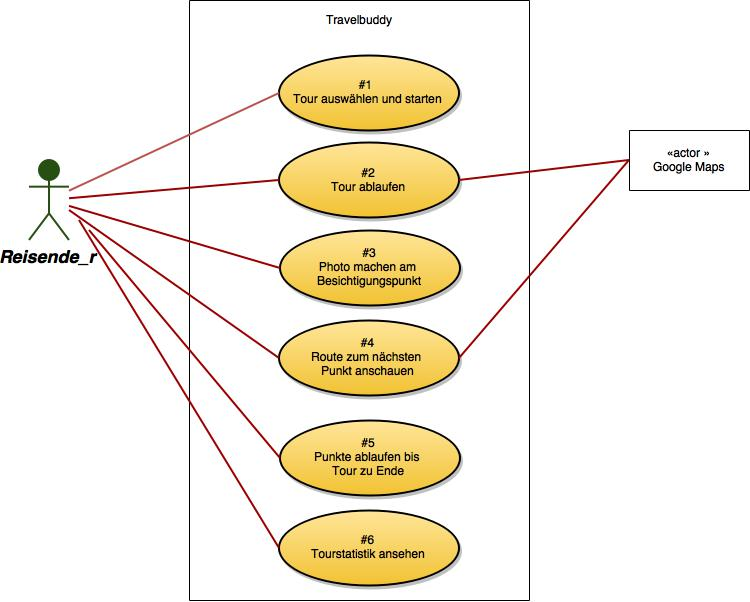
\includegraphics{docs/diagrams/Anwendungsfalldiagramm.jpg}
\caption{Anwendungsfalldiagramm}
\end{figure}

\section{Domänenmodell}\label{domuxe4nenmodell}

Das folgende Domänenmodell zeigt eine grobe Übersicht der Ausgangslage,
der identifizierten Objekte und Tätigkeiten der Benutzer.

\begin{figure}
\centering
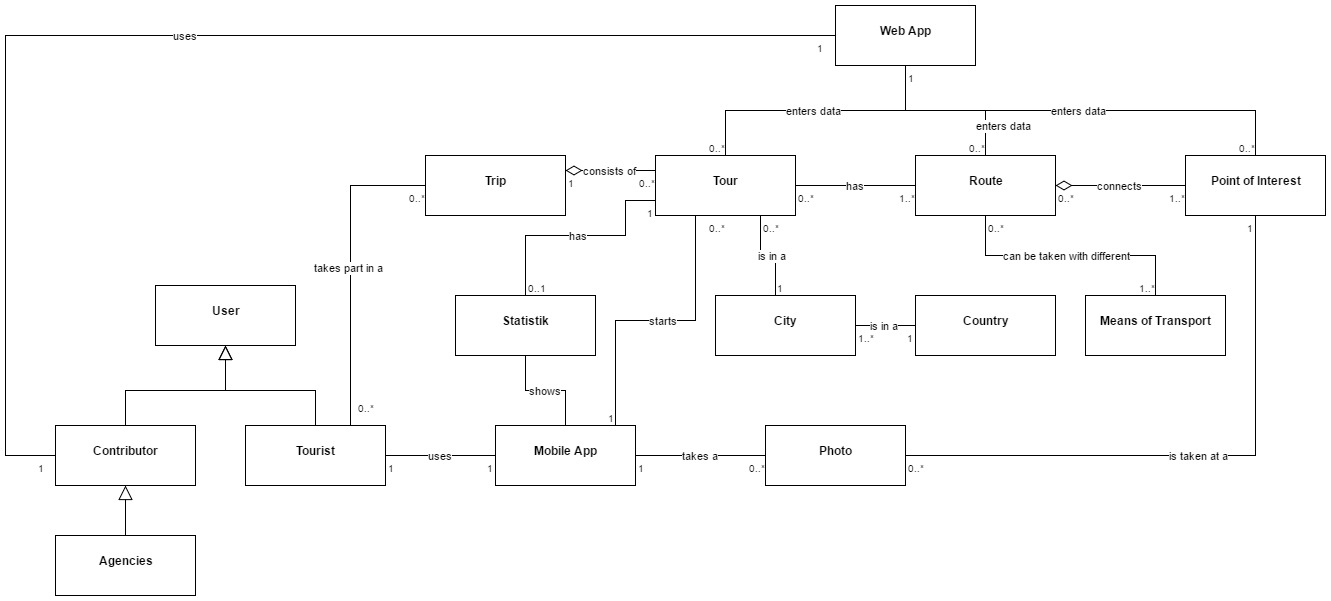
\includegraphics{https://raw.githubusercontent.com/PsitTeam3/Documentation/master/docs/diagrams/domain_model1.jpg}
\caption{Domain\_Model}
\end{figure}

\begin{longtable}[]{@{}ll@{}}
\toprule
\begin{minipage}[b]{0.08\columnwidth}\raggedright\strut
\textbf{Objekte}\strut
\end{minipage} & \begin{minipage}[b]{0.86\columnwidth}\raggedright\strut
\textbf{Beschreibung}\strut
\end{minipage}\tabularnewline
\midrule
\endhead
\begin{minipage}[t]{0.08\columnwidth}\raggedright\strut
User\strut
\end{minipage} & \begin{minipage}[t]{0.86\columnwidth}\raggedright\strut
Ein Benutzer kann in zwei verschiedenen Rollen auftreten. Als
\textbf{Contributor} oder \textbf{Tourist} auftreten.\strut
\end{minipage}\tabularnewline
\begin{minipage}[t]{0.08\columnwidth}\raggedright\strut
Contributor / Agencies\strut
\end{minipage} & \begin{minipage}[t]{0.86\columnwidth}\raggedright\strut
Ein \textbf{Contributor} erstellt und erfasst Inhalt (d.h.:
\textbf{Touren}, \textbf{Routen} und \textbf{Point of Interests}). Ein
Subtyp davon sind \textbf{Agencies}, also Reisebüros und
Tourismusorganisationen), die als zertifizierte Erfasser agieren.\strut
\end{minipage}\tabularnewline
\begin{minipage}[t]{0.08\columnwidth}\raggedright\strut
Tourist\strut
\end{minipage} & \begin{minipage}[t]{0.86\columnwidth}\raggedright\strut
Ein \textbf{Tourist} ist der eigentliche Benutzer der,App. Er ist auf
Reisen (\textbf{Trip}) und möchte an einem Ort bzw. in einer,Stadt eine
\textbf{Tour} unternehmen, um die wichtigsten oder spannendsten
\textbf{Point of Interest} kennen zu lernen. Er verwendet dafür die
\textbf{Mobile App}.\strut
\end{minipage}\tabularnewline
\begin{minipage}[t]{0.08\columnwidth}\raggedright\strut
Mobile App\strut
\end{minipage} & \begin{minipage}[t]{0.86\columnwidth}\raggedright\strut
Das ganze Applikations-System ist in zwei Komponenten aufgeteilt. Die
\textbf{Mobile App} wird vom \textbf{Touristen} verwendet um sich damit
unterstützt entlang einer \textbf{Tour} steuern zu lassen.\strut
\end{minipage}\tabularnewline
\begin{minipage}[t]{0.08\columnwidth}\raggedright\strut
Web App\strut
\end{minipage} & \begin{minipage}[t]{0.86\columnwidth}\raggedright\strut
Die \textbf{Web App} bietet die funktionale Schnittstelle für
\textbf{Contributors}.\strut
\end{minipage}\tabularnewline
\begin{minipage}[t]{0.08\columnwidth}\raggedright\strut
Trip\strut
\end{minipage} & \begin{minipage}[t]{0.86\columnwidth}\raggedright\strut
Ein \textbf{Tourist} macht eine Reise und hat dort je nach Ort und Stadt
mehrere verschiedene \textbf{Touren} zur Auswahl.\strut
\end{minipage}\tabularnewline
\begin{minipage}[t]{0.08\columnwidth}\raggedright\strut
Tour\strut
\end{minipage} & \begin{minipage}[t]{0.86\columnwidth}\raggedright\strut
Eine \textbf{Tour} ist eine Sammlung von \textbf{Point of Interest}s in
einer bestimmten \textbf{Stadt}, die über eine bestimmte \textbf{Route}
miteinander verbunden sind.\strut
\end{minipage}\tabularnewline
\begin{minipage}[t]{0.08\columnwidth}\raggedright\strut
Route\strut
\end{minipage} & \begin{minipage}[t]{0.86\columnwidth}\raggedright\strut
Eine \textbf{Route} stellt eine Verbindung von mehreren \textbf{Point of
Interests} dar. Eine Route kann mit verschiedenen
\textbf{Verkehrsmitteln} absolviert werden.\strut
\end{minipage}\tabularnewline
\begin{minipage}[t]{0.08\columnwidth}\raggedright\strut
Point of Interest\strut
\end{minipage} & \begin{minipage}[t]{0.86\columnwidth}\raggedright\strut
\textbf{Point of Interest} sind geographische Punkte, die eine
Sehenswürdigkeit oder sonstige spezielle Eigenschaften bieten. Sie
werden von einer \textbf{Route} verbunden. Der Tourist muss beim
Absolvieren einer Route an jedem \textbf{Point of Interest} vorbeikommen
und ein Foto schiessen.\strut
\end{minipage}\tabularnewline
\begin{minipage}[t]{0.08\columnwidth}\raggedright\strut
Means of Transport\strut
\end{minipage} & \begin{minipage}[t]{0.86\columnwidth}\raggedright\strut
Verschiedene \textbf{Verkehrsmittel} z.B.: ÖV, Auto, Velo, zu Fuss
usw\ldots{}\strut
\end{minipage}\tabularnewline
\begin{minipage}[t]{0.08\columnwidth}\raggedright\strut
Photo\strut
\end{minipage} & \begin{minipage}[t]{0.86\columnwidth}\raggedright\strut
An jedem \textbf{Point of Interest} schiesst der Benutzer mit seiner
\textbf{Mobile App} ein \textbf{Foto} des Ortes oder der
Sehenswürdigkeit. Die Koordinaten werden abgeglichen und der
\textbf{Point of Interest} so als besucht abgehakt.\strut
\end{minipage}\tabularnewline
\begin{minipage}[t]{0.08\columnwidth}\raggedright\strut
Statistik\strut
\end{minipage} & \begin{minipage}[t]{0.86\columnwidth}\raggedright\strut
Am Ende einer \textbf{Tour}, nachdem alle \textbf{Points of Interest},
besucht wurden, wird dem \textbf{Touristen} eine \textbf{Statistik} über
seine absolvierte \textbf{Route}, Anzahl Schritte, Distanz usw\ldots{}
angezeigt. Diese ist in der \textbf{Mobile App} verknüpft mit seinen
geschossen \textbf{Fotos}.\strut
\end{minipage}\tabularnewline
\bottomrule
\end{longtable}

\newpage

REVIEW by Raffaele

\section{Eine erste Architektur}\label{eine-erste-architektur}

Die Applikation besitzt mehrere Hauptkomponenten: • Mobile Application •
Web Service • External Services • Web Application Die Web Application
wurde zur besseren Gesamtübersicht in die Darstellung integriert, ist
aber nicht Bestandteil der Projekt-Umsetzung und wird daher auch nicht
detaillierter beschrieben.

\begin{figure}
\centering
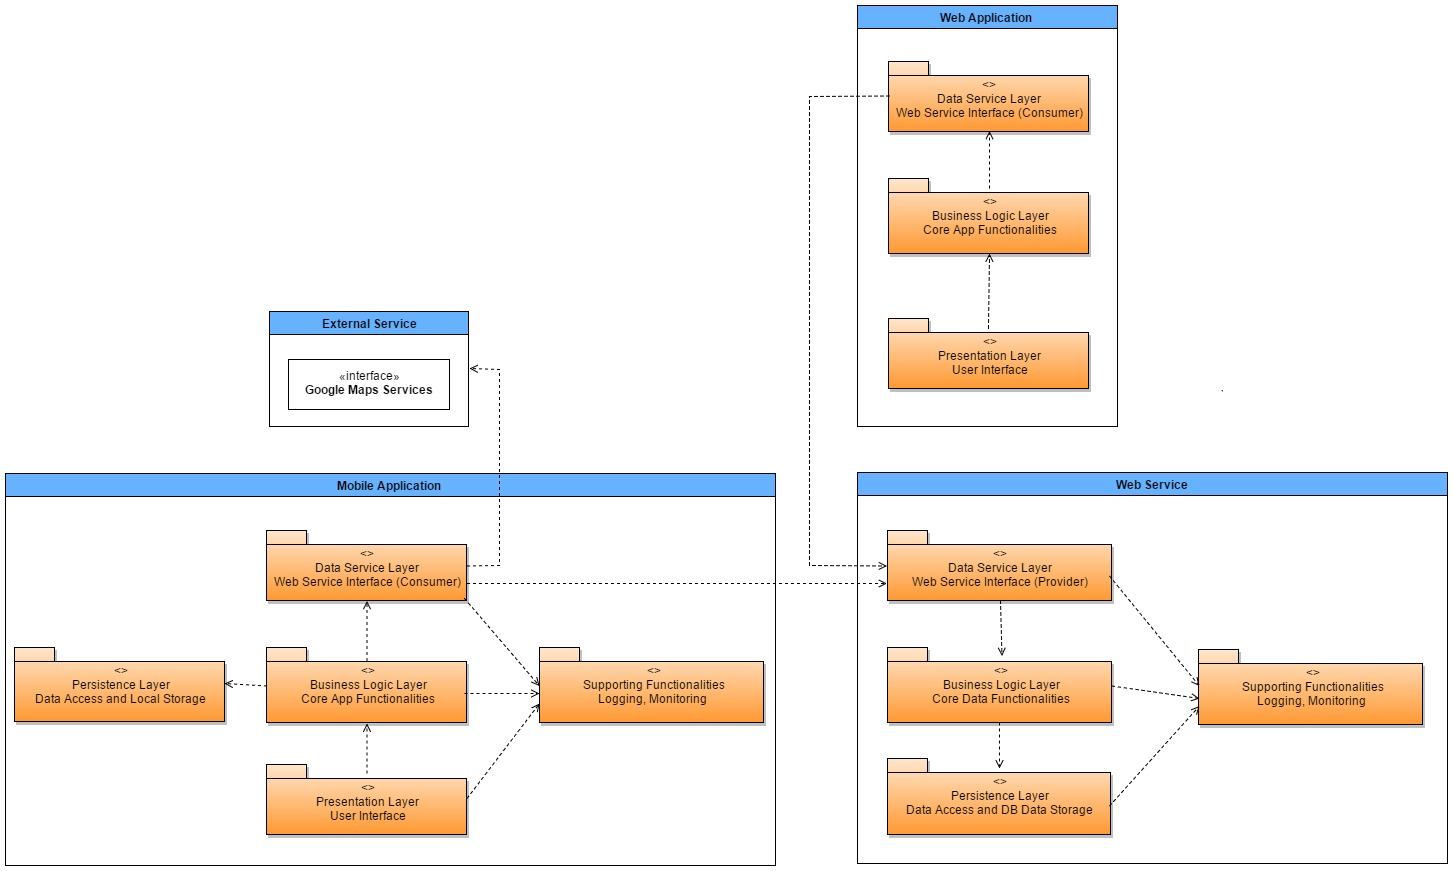
\includegraphics{https://raw.githubusercontent.com/PsitTeam3/Documentation/master/docs/diagrams/first_architecture1.jpg}
\caption{First\_Architecture}
\end{figure}

\textbf{Mobile Application:} Die Mobile Application wird vom Touristen
verwendet und bietet die Schnittstelle zu den eigentlichen
Hauptfunktionalitäten. Die App wird als 3-tier Applikation aufgebaut. Da
die Daten, auch für eine allfällig zukünftige offline-fähigkeit, sowohl
lokal in der App wie auch über die Data-Services persistiert werden bzw.
zum Beispiel Fotos nur lokal gespeichert werden, teilt sich der
Datenzugriffs-Layer, auf den Persistence Layer und den Data Service
Layer auf. Als vertikaler Layer werden für alle anderen Layer Logging-,
Monitoring- und weitere allgemein verwendete Funktionalitäten zur
Verfügung gestellt.

\begin{longtable}[]{@{}ll@{}}
\toprule
\begin{minipage}[b]{0.08\columnwidth}\raggedright\strut
\textbf{Komponente}\strut
\end{minipage} & \begin{minipage}[b]{0.86\columnwidth}\raggedright\strut
\textbf{Beschreibung}\strut
\end{minipage}\tabularnewline
\midrule
\endhead
\begin{minipage}[t]{0.08\columnwidth}\raggedright\strut
Presentation Layer\strut
\end{minipage} & \begin{minipage}[t]{0.86\columnwidth}\raggedright\strut
Implementiert die grafische Schnittstelle zum Benutzer. Weist neben
rudimentärer Eingabe- und Steuerungslogik, neben der Darstellung keine
weiteren Funktionalitäten auf.\strut
\end{minipage}\tabularnewline
\begin{minipage}[t]{0.08\columnwidth}\raggedright\strut
Business Logic Layer\strut
\end{minipage} & \begin{minipage}[t]{0.86\columnwidth}\raggedright\strut
Hier werden alle App-spezifischen Funktionalitäten implementiert. Dies
beinhaltet zum Beispiel das grafische Aufbereiten der erhaltenen Daten.
Anderseits sind Grundfunktionalitäten wie das Abgleichen der aktuellen
Position mit dem Point of Interest nicht Bestandteil dieses Layer,
sondern serverseitig umgesetzt werden.\strut
\end{minipage}\tabularnewline
\begin{minipage}[t]{0.08\columnwidth}\raggedright\strut
Persistence Layer\strut
\end{minipage} & \begin{minipage}[t]{0.86\columnwidth}\raggedright\strut
Der Persistence Layer bietet den Datenzugriff auf den lokalen Storage
der App. Damit werden zum Beispiel Fotos gespeichert.\strut
\end{minipage}\tabularnewline
\begin{minipage}[t]{0.08\columnwidth}\raggedright\strut
Data Service Layer\strut
\end{minipage} & \begin{minipage}[t]{0.86\columnwidth}\raggedright\strut
Dieser Layer bietet den Zugriff auf unseren eigenen Web-Daten-Service,
wie auch auf die Google Maps Services zum Anzeigen der Karte und
Berechnen der Route.\strut
\end{minipage}\tabularnewline
\begin{minipage}[t]{0.08\columnwidth}\raggedright\strut
Supporting Functionalities\strut
\end{minipage} & \begin{minipage}[t]{0.86\columnwidth}\raggedright\strut
Diese Komponente implementiert alle Funktionalitäten, die den anderen
Komponenten zur Verfügung stehen wie zum Beispiel Logging und sonstige
Monitoring-Funktionalitäten.\strut
\end{minipage}\tabularnewline
\bottomrule
\end{longtable}

\textbf{Web Service:} Der Webservice stellt als Backend-Komponente
sowohl Daten- wie auch funktionale Schnittstelle zur App und zu allen
weiteren Systemen oder externen Systemen dar. Er stellt jederzeit den
aktuellen Referenzdatenstand und alle grundlegenden nicht
zugriffs-system-spezifischen Funktionalitäten an. Dadurch kann eine hohe
Datenqualität und Datenkonsistenz sichergestellt werden. Der Web Service
muss hierfür eine Datenbank-Anbindung zur Persistierung der Daten
aufweisen. Genauso wie die Mobile Application wird der Web Service einen
vertikalen Layer für Logging-, Monitoring- und weitere allgemein
verwendete Funktionalitäten implementieren.

\begin{longtable}[]{@{}ll@{}}
\toprule
\begin{minipage}[b]{0.11\columnwidth}\raggedright\strut
\textbf{Komponente}\strut
\end{minipage} & \begin{minipage}[b]{0.83\columnwidth}\raggedright\strut
\textbf{Beschreibung}\strut
\end{minipage}\tabularnewline
\midrule
\endhead
\begin{minipage}[t]{0.11\columnwidth}\raggedright\strut
Data Service Layer\strut
\end{minipage} & \begin{minipage}[t]{0.83\columnwidth}\raggedright\strut
Der Data Service Layer stellt das nach aussen öffentlich verfügbare
Interface zur Verfügung. Er loggt und behandelt ankommende
Requests.\strut
\end{minipage}\tabularnewline
\begin{minipage}[t]{0.11\columnwidth}\raggedright\strut
Business Logic Layer\strut
\end{minipage} & \begin{minipage}[t]{0.83\columnwidth}\raggedright\strut
Dieser Layer besitzt alle Business-Funktionalitäten, die nicht reine
daten-spezifische Aggregation sind, wie zum Beispiel den Check, ob eine
Koordinate innerhalb eines Points of Interests ist.\strut
\end{minipage}\tabularnewline
\begin{minipage}[t]{0.11\columnwidth}\raggedright\strut
Persistence Layer\strut
\end{minipage} & \begin{minipage}[t]{0.83\columnwidth}\raggedright\strut
Implementiert sowohl den eigentlichen Datenzugriff, wie auch die
OR-Mapping Logik. Der Layer ist für einen konsistenten, Schreib- und
Lesezugriff auch bei mehreren gleichzeitigen abgearbeiteten Requests
verantwortlich.\strut
\end{minipage}\tabularnewline
\begin{minipage}[t]{0.11\columnwidth}\raggedright\strut
Supporting Functionalities\strut
\end{minipage} & \begin{minipage}[t]{0.83\columnwidth}\raggedright\strut
Diese Komponente implementiert alle Funktionalitäten, die den anderen
Komponenten zur Verfügung stehen wie zum Beispiel Logging und sonstige
Monitoring-Funktionalitäten.\strut
\end{minipage}\tabularnewline
\bottomrule
\end{longtable}

\textbf{External Services:} Wo bereits Funktionen oder grafische
Komponenten bestehen, werden diese über externe Services bezogen und
eingebunden. Hierbei werden wir in einem ersten Schritt auf öffentlich
zur Verfügung stehende Services zurückgreifen. Als grundlegenden Service
werden die Google Maps Funktionalitäten eingebunden.

Google Maps Services: Die Funktionalitäten zur Anzeige der Karte, den
verschiedenen Point of Interests und zur Berechnung der Route werden
nicht selber implementiert. Hierfür binden wir als externen Service die
Google Maps Services ein. Die Route und die Point of Interests, die vom
eigenen Web-Service geladen werden, werden als Overlay über die
Kartenfunktionalität von Google implementiert.

\textbf{Tech Stack:}

Die nachfolgende Tabelle zeigt die eingesetzten Technologien für die
einzelnen System-Komponenten. Innerhalb dieses Projekt-Scopes wird die
Mobile App als native Android App umgesetzt.

\begin{longtable}[]{@{}ll@{}}
\toprule
\begin{minipage}[b]{0.14\columnwidth}\raggedright\strut
\textbf{Komponente}\strut
\end{minipage} & \begin{minipage}[b]{0.80\columnwidth}\raggedright\strut
\textbf{Stack}\strut
\end{minipage}\tabularnewline
\midrule
\endhead
\begin{minipage}[t]{0.14\columnwidth}\raggedright\strut
Native Android App\strut
\end{minipage} & \begin{minipage}[t]{0.80\columnwidth}\raggedright\strut
JAVA 8Android SDK / Android Studio 2.3\strut
\end{minipage}\tabularnewline
\begin{minipage}[t]{0.14\columnwidth}\raggedright\strut
Web Service\strut
\end{minipage} & \begin{minipage}[t]{0.80\columnwidth}\raggedright\strut
.NET Framework 4.5C\# 5.0ASP.NET Web-API 2.2 (5.2.3)Entity Framework
6.0Ninject Dependency Injection Framework 3.2\strut
\end{minipage}\tabularnewline
\begin{minipage}[t]{0.14\columnwidth}\raggedright\strut
Web Application\strut
\end{minipage} & \begin{minipage}[t]{0.80\columnwidth}\raggedright\strut
.NET Framework 4.5C\# 5.0ASP.NET MVC 5.2.3 (Razor Engine)HTML 5.0Angular
JS 2.2.4 or React JS 15.4.2JQuery 3.2.1\strut
\end{minipage}\tabularnewline
\bottomrule
\end{longtable}

REVIEW by Josef

\section{Zusätzliche
Spezifikationen}\label{zusuxe4tzliche-spezifikationen}

\subsection{Einführung}\label{einfuxfchrung}

Hier werden hauptsächlich alle nicht funktionalen Anforderungen
definiert. Die funktionalen Anforderungen sind zum grössten Teil in den
Anwendungsfällen erfasst. An diesem Dokument finden sich nur weitere
funktionale Anforderungen, welche nicht in Zusammenhang mit einem
Anwendungsfall stehen.

\subsection{Funktionalität}\label{funktionalituxe4t}

\subsubsection{Logging /
Fehlerbehandlung}\label{logging-fehlerbehandlung}

Benutzer- und Systemaktivitäten sollen lokal auf dem Gerät gespeichert
werden. Im Fehlerfall können diese Informationen an den Server geschickt
und für die Fehleranalyse verwendet werden. Fehlerinformationen sollen
automatisch an den Server geschickt werden.

\subsubsection{Kartenmaterial}\label{kartenmaterial}

Für die Wegweisung soll die Kartenfunktionalität von Google verwendet
werden. Google Maps unterstützt das offline Speichern von bestimmten
Kartenabschnitten, was für Travelbuddy benötigt wird.

\subsubsection{Sicherheit}\label{sicherheit}

Um Touren durchführen zu können, muss sich die Kundin authentifizieren.
Dazu kann der Kunde ein Konto anlegen, oder sich mit seinem Facebook-
oder Google-Konto anmelden.

\subsection{Verwendbarkeit}\label{verwendbarkeit}

\subsubsection{Hardware Limitierung}\label{hardware-limitierung}

Die Applikation soll als Touchscreen-App für Android Geräte entwickelt
werden.

\subsubsection{Lokalisierung}\label{lokalisierung}

Verschiedene Sprachen müssen unterstützt werden können. Reisende wählen
ihre gewünschte Sprache in der App aus. Danach wird das GUI in der
vorgegebenen Sprache angezeigt. Die Touren werden ebenfalls in der
gewünschten Sprache angezeigt, sofern es eine Übersetzung gibt.

\subsubsection{Offline Unterstützung}\label{offline-unterstuxfctzung}

Die Tourensuche funktioniert nur, wenn der Kunde Internetzugang hat.
Einzelne Touren können danach lokal auf dem Gerät des Kunden gespeichert
werden, so dass Reisende eine Tour auch ohne Internetzugang durchführen
können.

\subsubsection{Graphische Oberfläche}\label{graphische-oberfluxe4che}

\begin{itemize}
\tightlist
\item
  Konzipiert für Smartphones und Tablets.
\item
  Bedienung durch Touchscreen.
\end{itemize}

\subsection{Umsetzungsbedingungen}\label{umsetzungsbedingungen}

Als Entwicklungsprozess wird der Unified Process verwendet. Dies ist ein
populärer, iterativer Software-Entwicklungsprozess um objektorientierte
Systeme zu bauen.\cite{UP}

\subsubsection{Backend}\label{backend}

Für die Umsetzung des Backends sollen folgende Microsoft Technologien
verwendet werden: * Microsoft ASP.NET * Microsoft SQL Server * Microsoft
Visual Studio 2015 Enterprise * .NET Framework 4.6

Das Backend stellt eine REST API bereit. Das Backend muss in der Lage
sein, Anfragen so schnell beantworten zu können, dass die Anforderungen
an das Reaktionsverhalten der App erfüllt werden können.

\begin{longtable}[]{@{}ll@{}}
\toprule
\begin{minipage}[b]{0.27\columnwidth}\raggedright\strut
Benutzer Aktion\strut
\end{minipage} & \begin{minipage}[b]{0.29\columnwidth}\raggedright\strut
Max. Reaktionszeit {[}ms{]}\strut
\end{minipage}\tabularnewline
\midrule
\endhead
\begin{minipage}[t]{0.27\columnwidth}\raggedright\strut
Anmelden\strut
\end{minipage} & \begin{minipage}[t]{0.29\columnwidth}\raggedright\strut
80\strut
\end{minipage}\tabularnewline
\begin{minipage}[t]{0.27\columnwidth}\raggedright\strut
Suchen nach Touren\strut
\end{minipage} & \begin{minipage}[t]{0.29\columnwidth}\raggedright\strut
150\strut
\end{minipage}\tabularnewline
\begin{minipage}[t]{0.27\columnwidth}\raggedright\strut
Starten von Touren\strut
\end{minipage} & \begin{minipage}[t]{0.29\columnwidth}\raggedright\strut
400\strut
\end{minipage}\tabularnewline
\begin{minipage}[t]{0.27\columnwidth}\raggedright\strut
Offline Speichern von Touren\strut
\end{minipage} & \begin{minipage}[t]{0.29\columnwidth}\raggedright\strut
Bandbreiten Abhängig. Daten \textless{} 10 MB\strut
\end{minipage}\tabularnewline
\begin{minipage}[t]{0.27\columnwidth}\raggedright\strut
Hochladen von Photos und Routenanzeige zum nächsten Standort\strut
\end{minipage} & \begin{minipage}[t]{0.29\columnwidth}\raggedright\strut
5000 (Photo komprimieren)\strut
\end{minipage}\tabularnewline
\bottomrule
\end{longtable}

\subsubsection{App}\label{app}

Es wird eine native Android Applikation entwickelt. Für die Entwicklung
wird verwendet: * Android Studio 2.3 * JetBrains IntelliJ

\subsection{Zuverlässigkeit}\label{zuverluxe4ssigkeit}

Bei einem Absturtz der App, muss die Reisende nach einem Neustart die
aktuelle Tour weiterführen können. Die App kennt den aktuellen Standort
und rekonstruiert gegebenenfalls die Route zum nächsten Ziel
vollautomatisch.

\section{Systemsequenzdiagram}\label{systemsequenzdiagram}

\begin{figure}
\centering
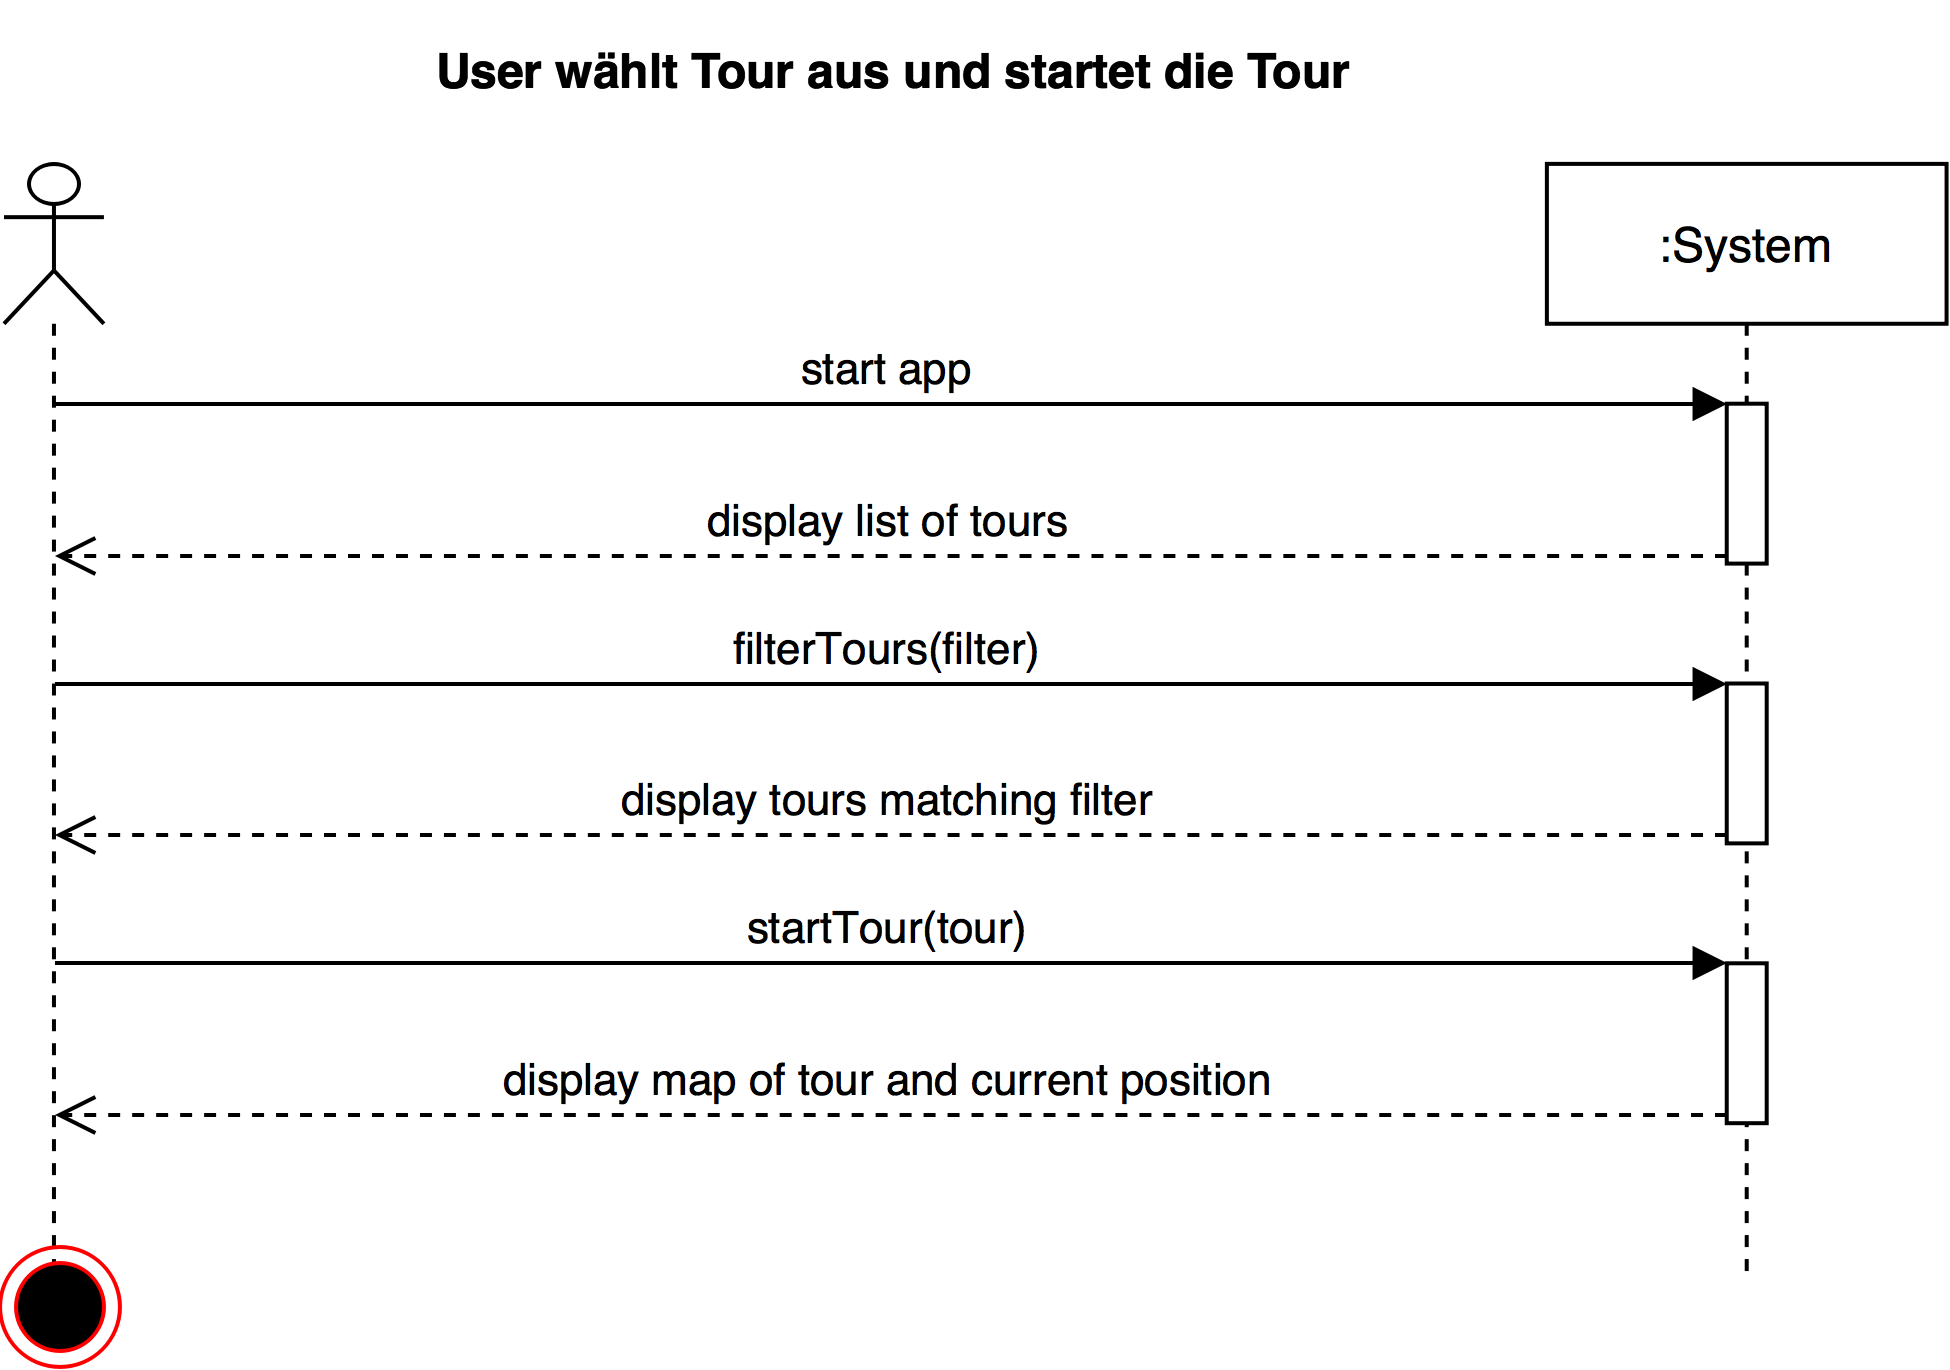
\includegraphics{docs/diagrams/UC1_SystemSequenzDiagram.png}
\caption{System Sequenz Diagramm}
\end{figure}

\section{Glossar}\label{glossar}

\begin{longtable}[]{@{}rl@{}}
\toprule
\begin{minipage}[b]{0.18\columnwidth}\raggedleft\strut
\textbf{Begriff}\strut
\end{minipage} & \begin{minipage}[b]{0.76\columnwidth}\raggedright\strut
\textbf{Erklärung}\strut
\end{minipage}\tabularnewline
\midrule
\endhead
\begin{minipage}[t]{0.18\columnwidth}\raggedleft\strut
Agency/Agencies\strut
\end{minipage} & \begin{minipage}[t]{0.76\columnwidth}\raggedright\strut
engl. Agenturen\strut
\end{minipage}\tabularnewline
\begin{minipage}[t]{0.18\columnwidth}\raggedleft\strut
API\strut
\end{minipage} & \begin{minipage}[t]{0.76\columnwidth}\raggedright\strut
Application Programming Interface, eine Schnittstelle zwischen zwei
Programmen\strut
\end{minipage}\tabularnewline
\begin{minipage}[t]{0.18\columnwidth}\raggedleft\strut
App\strut
\end{minipage} & \begin{minipage}[t]{0.76\columnwidth}\raggedright\strut
Abkz. Applikation, Synonym für Programm\strut
\end{minipage}\tabularnewline
\begin{minipage}[t]{0.18\columnwidth}\raggedleft\strut
Backend\strut
\end{minipage} & \begin{minipage}[t]{0.76\columnwidth}\raggedright\strut
Serverseitiges Programm das vom Benutzer nur über ein Frontend
angesteuert werden kann\strut
\end{minipage}\tabularnewline
\begin{minipage}[t]{0.18\columnwidth}\raggedleft\strut
Business Logic\strut
\end{minipage} & \begin{minipage}[t]{0.76\columnwidth}\raggedright\strut
engl. Geschäftslogik, logischer Ablauf des Programmes\strut
\end{minipage}\tabularnewline
\begin{minipage}[t]{0.18\columnwidth}\raggedleft\strut
Construction-phase\strut
\end{minipage} & \begin{minipage}[t]{0.76\columnwidth}\raggedright\strut
Phase in der das Projekt umgesetzt wird\strut
\end{minipage}\tabularnewline
\begin{minipage}[t]{0.18\columnwidth}\raggedleft\strut
Contributor\strut
\end{minipage} & \begin{minipage}[t]{0.76\columnwidth}\raggedright\strut
engl. Beitragender, jemand der Inhalt für die Applikation erstellt\strut
\end{minipage}\tabularnewline
\begin{minipage}[t]{0.18\columnwidth}\raggedleft\strut
Elaboration-phase\strut
\end{minipage} & \begin{minipage}[t]{0.76\columnwidth}\raggedright\strut
Phase in der das Projekt genauer ausgearbeitet wird\strut
\end{minipage}\tabularnewline
\begin{minipage}[t]{0.18\columnwidth}\raggedleft\strut
External Services\strut
\end{minipage} & \begin{minipage}[t]{0.76\columnwidth}\raggedright\strut
engl. Externe Dienste, Dienste die nicht vom Programm selber ausgeführt
werden\strut
\end{minipage}\tabularnewline
\begin{minipage}[t]{0.18\columnwidth}\raggedleft\strut
Fallback\strut
\end{minipage} & \begin{minipage}[t]{0.76\columnwidth}\raggedright\strut
Ausweichlösung/Alternativlösung\strut
\end{minipage}\tabularnewline
\begin{minipage}[t]{0.18\columnwidth}\raggedleft\strut
Frontend\strut
\end{minipage} & \begin{minipage}[t]{0.76\columnwidth}\raggedright\strut
Benutzerseitiges Programm das vom Benutzer direkt gesteuert werden
kann\strut
\end{minipage}\tabularnewline
\begin{minipage}[t]{0.18\columnwidth}\raggedleft\strut
GPS\strut
\end{minipage} & \begin{minipage}[t]{0.76\columnwidth}\raggedright\strut
Globa Positioning System, globales Satelliten Navigationsnetz\strut
\end{minipage}\tabularnewline
\begin{minipage}[t]{0.18\columnwidth}\raggedleft\strut
Inception-phase\strut
\end{minipage} & \begin{minipage}[t]{0.76\columnwidth}\raggedright\strut
Gründungsphase, beginn des Projektes\strut
\end{minipage}\tabularnewline
\begin{minipage}[t]{0.18\columnwidth}\raggedleft\strut
Logging\strut
\end{minipage} & \begin{minipage}[t]{0.76\columnwidth}\raggedright\strut
Aufzeichnen von Abläufen im Programm\strut
\end{minipage}\tabularnewline
\begin{minipage}[t]{0.18\columnwidth}\raggedleft\strut
Marker\strut
\end{minipage} & \begin{minipage}[t]{0.76\columnwidth}\raggedright\strut
Symbol das einen Punkt auf der Karte markiert\strut
\end{minipage}\tabularnewline
\begin{minipage}[t]{0.18\columnwidth}\raggedleft\strut
Means of Transport\strut
\end{minipage} & \begin{minipage}[t]{0.76\columnwidth}\raggedright\strut
engl. Verkehrsmittel\strut
\end{minipage}\tabularnewline
\begin{minipage}[t]{0.18\columnwidth}\raggedleft\strut
Meilenstein\strut
\end{minipage} & \begin{minipage}[t]{0.76\columnwidth}\raggedright\strut
Bedeutender Schritt in der Entwicklung\strut
\end{minipage}\tabularnewline
\begin{minipage}[t]{0.18\columnwidth}\raggedleft\strut
Mobile App\strut
\end{minipage} & \begin{minipage}[t]{0.76\columnwidth}\raggedright\strut
Programm dass nur auf einem Mobilgerät ausgeführt werden kann\strut
\end{minipage}\tabularnewline
\begin{minipage}[t]{0.18\columnwidth}\raggedleft\strut
Native\strut
\end{minipage} & \begin{minipage}[t]{0.76\columnwidth}\raggedright\strut
Funktionen die von einem Gerät ohne weitere Software ausgeführt werden
kann\strut
\end{minipage}\tabularnewline
\begin{minipage}[t]{0.18\columnwidth}\raggedleft\strut
ÖV\strut
\end{minipage} & \begin{minipage}[t]{0.76\columnwidth}\raggedright\strut
abkz. Öffentlicher Verkehr\strut
\end{minipage}\tabularnewline
\begin{minipage}[t]{0.18\columnwidth}\raggedleft\strut
Point of Interest, PoI\strut
\end{minipage} & \begin{minipage}[t]{0.76\columnwidth}\raggedright\strut
engl. Ort von besonderem Interesse, bspw. Wahrzeichen\strut
\end{minipage}\tabularnewline
\begin{minipage}[t]{0.18\columnwidth}\raggedleft\strut
Ressource\strut
\end{minipage} & \begin{minipage}[t]{0.76\columnwidth}\raggedright\strut
Mittel das zur Entwicklung genutzt werden kann\strut
\end{minipage}\tabularnewline
\begin{minipage}[t]{0.18\columnwidth}\raggedleft\strut
Smartphone\strut
\end{minipage} & \begin{minipage}[t]{0.76\columnwidth}\raggedright\strut
Mobilgerät mit erweiterten Funktionen\strut
\end{minipage}\tabularnewline
\begin{minipage}[t]{0.18\columnwidth}\raggedleft\strut
Stakeholders\strut
\end{minipage} & \begin{minipage}[t]{0.76\columnwidth}\raggedright\strut
engl. Interessenten\strut
\end{minipage}\tabularnewline
\begin{minipage}[t]{0.18\columnwidth}\raggedleft\strut
Tech Stack\strut
\end{minipage} & \begin{minipage}[t]{0.76\columnwidth}\raggedright\strut
Eingesetzte Technologien\strut
\end{minipage}\tabularnewline
\begin{minipage}[t]{0.18\columnwidth}\raggedleft\strut
Trip\strut
\end{minipage} & \begin{minipage}[t]{0.76\columnwidth}\raggedright\strut
engl. Reise\strut
\end{minipage}\tabularnewline
\begin{minipage}[t]{0.18\columnwidth}\raggedleft\strut
Use-Case\strut
\end{minipage} & \begin{minipage}[t]{0.76\columnwidth}\raggedright\strut
engl. Anwendungsfall, Szenarien in der ein Benutzer versucht ein
bestimmtes Ziel zu erreichen\strut
\end{minipage}\tabularnewline
\begin{minipage}[t]{0.18\columnwidth}\raggedleft\strut
User\strut
\end{minipage} & \begin{minipage}[t]{0.76\columnwidth}\raggedright\strut
engl. Benutzer\strut
\end{minipage}\tabularnewline
\begin{minipage}[t]{0.18\columnwidth}\raggedleft\strut
Web App\strut
\end{minipage} & \begin{minipage}[t]{0.76\columnwidth}\raggedright\strut
Nur über den Webbrowser benutzbares Programm\strut
\end{minipage}\tabularnewline
\begin{minipage}[t]{0.18\columnwidth}\raggedleft\strut
WLAN\strut
\end{minipage} & \begin{minipage}[t]{0.76\columnwidth}\raggedright\strut
Wireless local area netweork, Kabellose netzwerkverbindung\strut
\end{minipage}\tabularnewline
\bottomrule
\end{longtable}

REVIEW by Beni

\addcontentsline{toc}{section}{Literatur}\begin{thebibliography}{9}
\bibitem{UP}
C. Larman, Applying UML and patterns. 4. Auflage, Upper Saddle River: Pearson Education, Inc., 2005, S. 18.
\end{thebibliography}

\end{document}
